\chapter{Introduction}\label{ch:overview}
A crucial part of the T\&E Framework (TEF) is to log information during the operation of a lifelong learning system and use this to derive \textit{metrics of lifelong learning}, i.e., to characterize how well the system learns along the dimensions (Core Capabilities) set out in the DARPA L2M BAA, such as Continual Learning (CL) and Adaptation to New Tasks (ANT). This is termed the \textbf{Metrics Framework}.\\[0.2in]

\begin{figure}[h]
	\centering
	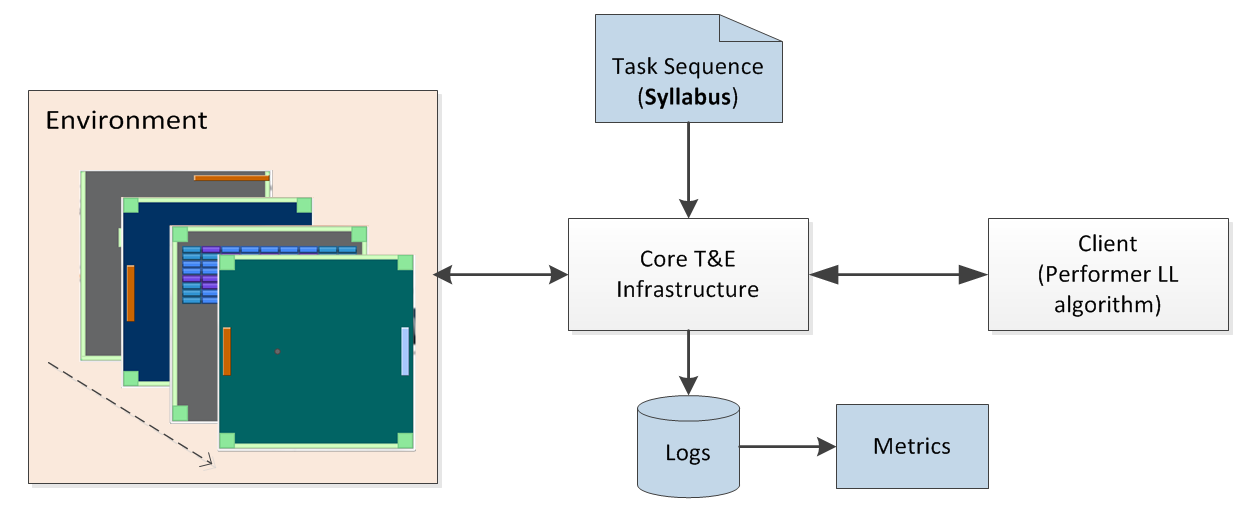
\includegraphics[width=0.8\columnwidth]{sections/figs/metrics_diagram.png}
	\caption{Depiction of the Metrics Framework}
	\label{fig:framework}
\end{figure}

\flushleft The Metrics Framework consists of three components:\\[0.2in]
\begin{enumerate}
\item \textit{Performance Logging.} As a learning algorithm goes through a syllabus, Learnkit automatically logs information about the performance of the learning algorithm. For Agent learning, the logged information consists of the total reward for each episode; for classification learning, the logged information consists of the performance error on each batch (the definition of “performance error” is task-specific).\\[0.1in]
\item \textit{Metrics Calculation.} After the training is completed, the performance logs are read and processed by a separate L2M Python package. This package (the l2metrics repository) consists of a set of predefined metrics, and a Python class hierarchy for extending the predefined set with custom metrics.\\[0.1in]
\item \textit{Syllabus Annotation.} The metrics calculation assumes that the Learnkit syllabus has specific annotations (e.g., to distinguish training vs. test phases, or different parts of a test phase); relatedly, different syllabi may exercise different aspects of lifelong learning, such as Continual Learning versus Adapting to New Tasks. Consequently, authoring correctly-annotated syllabi is a crucial component of the Metrics Framework.\\[0.2in]
\end{enumerate}
    
The following table summarizes the different ways in which we anticipate performers will engage with the Metrics Framework. 

\begin{table}[h]
\begin{tabular}{|l|l|}
\hline
\textbf{Goal:}                                                                              & \textbf{Relevant Section:} \\ \hline
\begin{tabular}[c]{@{}l@{}}Generate metrics for a syllabus. Run an L2 algorithm\\ using a predefined syllabus, run the predefined metrics,\\ and view the results\end{tabular} & 3. Generating Metrics for a Syllabus\\\hline                                                                              
\begin{tabular}[c]{@{}l@{}}Create a custom syllabus. Run an L2 algorithm with a\\custom syllabus, and run predefined metrics.\end{tabular} & 4. Creating Custom Syllabi\\\hline         
\begin{tabular}[c]{@{}l@{}}Create a custom metric. Run an L2 algorithm with a\\predefined or custom syllabus, and run a custom metric.\end{tabular} & \begin{tabular}[c]{@{}l@{}}4. Creating Custom Syllabi\\5. Creating Custom Metrics\end{tabular}\\ \hline
                                                                                  
\end{tabular}
\end{table}

\section{Conceptual Overview}

\subsection*{Agent Learning}

The T\&E Framework uses the information contained in an annotated syllabusto produce a sequence of specific tasks, known as episodes, for an agent learner and automaticallly generates the performance logs from which metrics will be calculated. Figure~\ref{fig:workflow} depicts the workflow of the system as described below.\\[0.2in]

\begin{figure}[h]
	\centering
	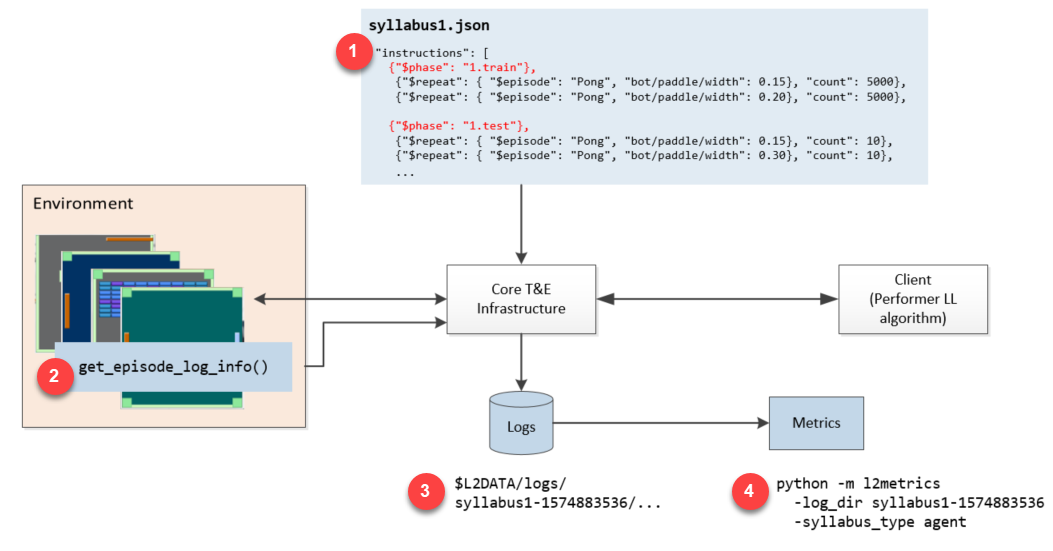
\includegraphics[width=0.9\columnwidth]{sections/figs/metrics_overview_1.png}
	\caption{Workflow in the Metrics Framework}
	\label{fig:workflow}
\end{figure}

\begin{enumerate}
\item The performance logging starts with an annotated syllabus (see Figure~\ref{fig:annotated_syllabus} for an example). The annotation consists of the “\$phase” instructions; the phase values (e.g., “1.train”) have a specific structure that is used during the metrics calculation.\\[0.4in]

\begin{figure}[h]
	\centering
	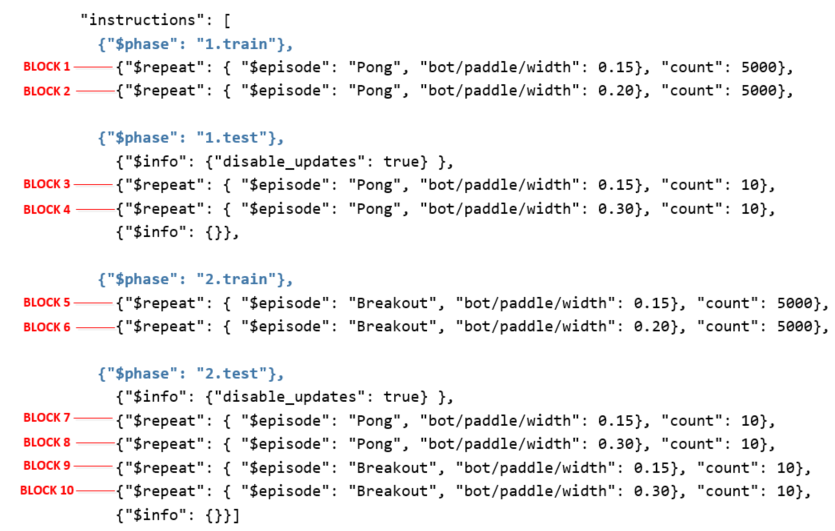
\includegraphics[width=0.8\columnwidth]{sections/figs/syllabus_annotated_blocks.png}
	\caption{An Annotated Syllabus Example}
	\label{fig:annotated_syllabus}
\end{figure}


\item Tasks in the L2M environment (such as Pong L2Arcade, or L2StarCraft CollectThings) have a special method (
\begin{small}
\verb|get_episode_log_info| 
\end{small}
) that reports the total reward and related performance information for each episode. This is automatically called by Learnkit as the syllabus is processed; performer code does not need to do anything (and in particular, the performer algorithm should not call 
\begin{small}
\verb|get_episode_log_info| 
\end{small}
or use the information reported therein).\\[0.1in]

\item The performance logs from running the syllabus are automatically saved under the L2M logging directory (the default value of the top-level logging directory is OS-specific, and it can be overridden using the \$L2DATA environment variable). The logs for running a specific syllabus are saved under a unique directory name <syllabus\_name>-<timestamp>.The
\begin{small}
\verb|python -m learnkit.info|
\end{small}
command shows the location of the directory, along with the most recently created log directory:\\[0.1in]

\begin{small}
\begin{verbatim}
bakermm1@bakermm1-ll2:~/L2M/l2metrics$ python -m learnkit.info
Learnkit v0.5.0
L2 data folder:
   /home/bakermm1/l2data
L2 logs folder:
   /home/bakermm1/l2data/logs
Most recent log folder:
   /home/bakermm1/l2data/logs/syllabus_CL-1575473425723
   created on 2019-12-04T10:30:25
\end{verbatim}
\end{small}

Under \$L2DATA/logs/<syllabus\_name>-<timestamp>/ the directory tree looks like this: <worker\_id>/<phase\_name>/<task\_name>/{block-report, data-log}.tsv. A few points worth noting about this logging structure:\\[0.2in]
\begin{itemize}
\item The worker ID is for distributed training. The ordering of episodes is maintained across workers, so an episode number is unique across the distributed training.\\[0.1in]
\item The syllabus is notionally divided into a sequence of blocks; each block is a sequence of episodes with the same Task name and parameter values. See Figure~\ref{fig:annotated_syllabus} for an example.\\[0.1in]
\item Each episode consists of one or more sub-episodes (each sub-episode is a reset, followed by one or more steps). This is the granularity for the performance logging – for each sub-episode, the logs record the total reward and whether that sub-episode as complete (i.e., continued until done) or incomplete. \\[0.1in]
\item block-report.tsv contains metadata about each block. data-log.tsv contains the actual logged information about each episode and its sub-episodes. Note that in the logs, “task” and “sub\_task” specify the episode and sub-episode number, respectively.\\[0.1in]
\end{itemize}
\item Once the learning algorithm is done, the predefined metrics calculations can be invoked by specifying the directory of the log files, e.g.: \\[0.1in]
\end{enumerate}

\begin{small}
\begin{verbatim} python -m l2metrics  -log_dir syllabus1-1574883536 -syllabus_type agent \end{verbatim}
\end{small}

Conceptually, the above command loads the log data into a single data table, hands it to each Metric (a Python class), collects the results and prints them out. It is also possible to write a custom script with custom metrics and with full control over which metrics are calculated.

\subsection*{Classification Learning}

The logging for classification learning is conceptually similar to that for agent learning. The main difference is in what gets logged and at what granularity (corresponding to Workflow steps 2 and 3 in Figure~\ref{fig:framework}).\\[0.1in]

Recall that a Classification syllabus consists of a sequence of datasets; each dataset consists of one or batches; each batch is a sequence of examples; each example is one input to the learning agent, with an optional output or ground truth value. When performer code interacts a Classification Task (such as CIFAR100), the code looks something like this:

\begin{small}
\begin{verbatim} 
for dataset in syllabus.datasets():       
       dataset.reset()
       done = False
       while not done:
           batch, done, info = dataset.next_batch()
           y_hat = do_inference(batch['inputs'])  # performer code
           y = dataset.get_labels(batch[id'], y_hat)
           if y:
               calculate_loss_and_update_model(y, y_hat)  # performer code 
\end{verbatim}
\end{small}

Crucially, the performer code has to submit the estimated outputs
\begin{small}
\verb|y_hat|
\end{small}via the
\begin{small}
\verb|get_labels|
\end{small}method; this is done for both training and test data. The Classification Task uses this
\begin{small}
\verb|y_hat|
\end{small}to calculate the error for the batch, and has a special method
\begin{small}
\verb|get_batch_log_info|
\end{small}that reports the error information to Learnkit for logging. This method is automatically called by Learnkit as the syllabus is processed; performer code does not need to do anything, and in particular should not invoke
\begin{small}
\verb|get_batch_log_info.|
\end{small}This information is only intended for Learnkit logging; performers should use their own loss functions as appropriate for their models.

\section{Sample Workflow to Generate Metrics}

The following instuctions illustrate how to operate in the Metrics Framework in a sample environment called Minigrid. Please note that while we have adapted this environment to work with Learnkit, it will not be used for the T\&E Framework but serves as a quick-to-train example to generate log files in the proper format. After setting up the python packages (steps 1-3), an agent should be trained using the minigridkit script (step 4). Behind the scenes, this script uses Learnkit to load a Continual Learning syllabus which queues up sequences of episodes in which the agent can learn. While the agent is being fed these episodes, Learnkit automatically logs the reward achieved at the end of each episode and saves it to TSV files. The location of these files must be passed (step 5) to the l2metrics code, which computes Metrics and prints out the results (step 6). \\[0.2in]

\begin{enumerate}

\item Clone the learnkit repository\\
\begin{small}
\verb|pip install -e learnkit\|\\[0.1in]
\end{small}

\item Clone the minigridkit repository\\
\begin{small}
\verb|pip install -e minigridkit\|\\[0.1in]
\end{small}

\item Clone the l2metrics repository\\
\begin{small}
\verb|pip install -e l2metrics\|\\[0.1in]
\end{small}

\item Train an agent in the Minigrid environment. This will take a few minutes. When it starts you should see an INFO level message showing the top level directory where logs are being written.\\[0.1in]
\begin{small}
\verb|python minigrid_learnkit/examples/minigrid_train_ppo.py| \\
\verb|2019-12-04 10:30:25,723 <22980> | \\
\verb|[INFO    ] root - Logging to: /home/bakermm1/l2data/logs|\\[0.1in]
\end{small}

\item Store the last used logging directory in a temporary variable.\\
\begin{small}
\verb|log_dir =$(ls -t -1 `python -m learnkit.info -get logdir`| |\verb| head -1)|\\[0.1in]
\end{small}
\item Pass the variable just set as the 
\begin{small}
\verb|-log_dir|
\end{small}parameter when you run calc\_metrics\\
\begin{small}
\verb|cd l2metrics/examples|
\verb|python calc_metrics.py -syllabus_subtype=CL -log_dir=$log_dir|\\[0.2in]
\end{small}
\end{enumerate}
The output should print to the screen and should look something like this:\\[0.2in]

\begin{verbatim}

Metric: Average Within Block Saturation Calculation

Averaged Value: {'global_within_block_saturation': 0.875959925753812, 
                'global_num_eps_to_saturation': 197.45454545454547}
                
Per Block Values: {
'saturation_value': {0: 0.8488624196510561, 1: 0.822495598845599, 
2: 0.8413838383838385, 3: 0.9651983081298474, 4: 0.8791413586413588, 
5: 0.8132655122655124, 6: 0.8654549980322708, 7: 0.9549258642961517, 
8: 0.9681967251617378, 9: 0.8410522366522368, 10: 0.8355823232323233},

'eps_to_saturation': {0: 185, 1: 30, 2: 81, 3: 107, 4: 610, 5: 83, 
6: 84, 7: 100, 8: 739, 9: 103, 10: 50}}

Metric: An Example Custom Metric
Averaged Value: {'global_perf': 0.9217597535934293}
Per Block Values: {'global_perf': 0.9217597535934293}

Process finished with exit code 0

\end{verbatim}
